\documentclass[output=paper]{langscibook}
\ChapterDOI{10.5281/zenodo.15006617}

\author{Stefan Dollinger\orcid{}\affiliation{UBC Vancouver}}
\title[Dialectology as “language making”]{Dialectology as “language making”: Hegemonic disciplinary discourse and the One Standard German Axiom (OSGA)}
\subtitle{Hegemonic disciplinary discourse and the One Standard German Axiom (OSGA)}

\abstract{This paper problematizes the current anti-pluricentric perspectives in German dialectology in the context of “language making” \citep{KrämerEtAl2022}. Disciplinary history and cross-linguistic comparison shed light on what appears to be  discipline-internal theoretical hegemony on what makes a language and what a dialect. The paper proposes the existence of a long-standing, discipline-defining One Standard German Axiom (OSGA) to be operative, an axiom that “unmakes” non-dominant standard varieties. It will be shown that, given the unbroken chain of tradition in German dialectology (via, e.g. Kranzmayer or Mitzka) based on Germanic \textit{Stämme} (`tribes'), the concept of “German language” is a priori defined as a stand-alone single entity. A comparison between \textit{Stämme} in German literature~– now obsolete~– and \textit{Stämme} in German dialectology~–  still strong~– illustrates the far-reaching ramifications of OSGA. Three fail-safes are suggested to move the debate onto an epistemologically sounder footing and to allow for the dynamic, in part predictable, development of multiple linguistic standards in German via Pluricentric Theory (Multi-Standard Theory). Pluricentric Theory remains, it is argued, the theory of choice, though the present paper extends \citeauthor{Clyne1995}'s \citeyearpar{Clyne1995} model with transnational cross-linguistic influence.}
\IfFileExists{../localcommands.tex}{
  \addbibresource{../localbibliography.bib}
  \usepackage{tabularx,multicol}
%\usepackage{multirow}
\usepackage{subcaption}
\usepackage{url}
\urlstyle{same}

\usepackage{datetime}
\usepackage{enumitem}
\usepackage{langsci-optional}
\usepackage{langsci-lgr}
\usepackage{langsci-branding}

\usepackage{longtable}
\usepackage{xltabular}
\usepackage[linguistics, edges]{forest}
\usepackage{pgfplots}
\pgfplotsset{compat=1.18}
\usetikzlibrary{patterns, tikzmark}
\usepackage{pgfplotstable}
\usepgfplotslibrary{colorbrewer}
\usepackage{listings}
\lstset{basicstyle=\ttfamily,keywordstyle=\normalfont,language=,breaklines=true}

\usepackage{siunitx}
\sisetup{group-digits=none, detect-all=true}

\usepackage{langsci-gb4e}

  \makeatletter
\let\thetitle\@title
\let\theauthor\@author
\makeatother

% Use this Chinese font shipped with TeX Live instead of Source Han, because
% it is more portable/leightweight. Install the "fandol" package from CTAN to
% automatically get this font.
\newfontfamily{\ChineseFandolSong}{FandolSong-Regular.otf}

  %% hyphenation points for line breaks
%% Normally, automatic hyphenation in LaTeX is very good
%% If a word is mis-hyphenated, add it to this file
%%
%% add information to TeX file before \begin{document} with:
%% %% hyphenation points for line breaks
%% Normally, automatic hyphenation in LaTeX is very good
%% If a word is mis-hyphenated, add it to this file
%%
%% add information to TeX file before \begin{document} with:
%% %% hyphenation points for line breaks
%% Normally, automatic hyphenation in LaTeX is very good
%% If a word is mis-hyphenated, add it to this file
%%
%% add information to TeX file before \begin{document} with:
%% \include{localhyphenation}
\hyphenation{
    a-na-ly-sis
    ap-proach-es
    ar-che-o-log-i-cal
    Ar-khan-gelsk
    be-schrei-ben
    Buch-holtz
    Che-lya-binsk
    con-so-nant
    dia-lect
    dia-lect-ology
    Di-a-lekt-for-schung
    Dia-lekt-for-schung
    East-pha-lian
    För-der-ung
    Ge-mein-schaft-lich-keits-ent-wür-fe
    his-tor-i-cal
    Hok-kai-do
    ja-pa-nese
    Ja-pa-nese
    Ka-go-shi-ma
    Ka-li-nin-grad
    Knja-zev
    Ma-kro-be-reich
    Ma-lay-sia
    mor-pho-log-i-cal
    Mos-cow
    Nef-te-yu-gansk
    non-mobile
    nu-cle-ar
    ös-ter-rei-chi-sche
    par-a-digm
    per-zep-ti-ons-lin-gu-is-ti-sche
    plu-ri-zen-tri-schen
    quick-ly
    Reich
    Sax-on
    Schrö-der
    sear-ching
    ste-reo-type
    strength-en-ing
    strong-est
    Stutt-gart
    su-pra-seg-men-tal
    teach-er
    to-po-gra-phy
    To-ron-to
    tra-di-tion-al
    ul-ti-mate-ly
    Um-gangs-spra-che
    Volks-kun-de
    vor-zu-stel-len
    wheth-er
    Wie-sing-er
    with-in
    Wort-at-las
}

\hyphenation{
    a-na-ly-sis
    ap-proach-es
    ar-che-o-log-i-cal
    Ar-khan-gelsk
    be-schrei-ben
    Buch-holtz
    Che-lya-binsk
    con-so-nant
    dia-lect
    dia-lect-ology
    Di-a-lekt-for-schung
    Dia-lekt-for-schung
    East-pha-lian
    För-der-ung
    Ge-mein-schaft-lich-keits-ent-wür-fe
    his-tor-i-cal
    Hok-kai-do
    ja-pa-nese
    Ja-pa-nese
    Ka-go-shi-ma
    Ka-li-nin-grad
    Knja-zev
    Ma-kro-be-reich
    Ma-lay-sia
    mor-pho-log-i-cal
    Mos-cow
    Nef-te-yu-gansk
    non-mobile
    nu-cle-ar
    ös-ter-rei-chi-sche
    par-a-digm
    per-zep-ti-ons-lin-gu-is-ti-sche
    plu-ri-zen-tri-schen
    quick-ly
    Reich
    Sax-on
    Schrö-der
    sear-ching
    ste-reo-type
    strength-en-ing
    strong-est
    Stutt-gart
    su-pra-seg-men-tal
    teach-er
    to-po-gra-phy
    To-ron-to
    tra-di-tion-al
    ul-ti-mate-ly
    Um-gangs-spra-che
    Volks-kun-de
    vor-zu-stel-len
    wheth-er
    Wie-sing-er
    with-in
    Wort-at-las
}

\hyphenation{
    a-na-ly-sis
    ap-proach-es
    ar-che-o-log-i-cal
    Ar-khan-gelsk
    be-schrei-ben
    Buch-holtz
    Che-lya-binsk
    con-so-nant
    dia-lect
    dia-lect-ology
    Di-a-lekt-for-schung
    Dia-lekt-for-schung
    East-pha-lian
    För-der-ung
    Ge-mein-schaft-lich-keits-ent-wür-fe
    his-tor-i-cal
    Hok-kai-do
    ja-pa-nese
    Ja-pa-nese
    Ka-go-shi-ma
    Ka-li-nin-grad
    Knja-zev
    Ma-kro-be-reich
    Ma-lay-sia
    mor-pho-log-i-cal
    Mos-cow
    Nef-te-yu-gansk
    non-mobile
    nu-cle-ar
    ös-ter-rei-chi-sche
    par-a-digm
    per-zep-ti-ons-lin-gu-is-ti-sche
    plu-ri-zen-tri-schen
    quick-ly
    Reich
    Sax-on
    Schrö-der
    sear-ching
    ste-reo-type
    strength-en-ing
    strong-est
    Stutt-gart
    su-pra-seg-men-tal
    teach-er
    to-po-gra-phy
    To-ron-to
    tra-di-tion-al
    ul-ti-mate-ly
    Um-gangs-spra-che
    Volks-kun-de
    vor-zu-stel-len
    wheth-er
    Wie-sing-er
    with-in
    Wort-at-las
}

  \togglepaper[1]%%chapternumber
}{}

\begin{document}
\maketitle
\label{chap:dollinger}
\graphicspath{{figures/dollinger}}


\section{Dialectology as language making: Past and present}
\label{sec:dollinger:1}
While the problem of objectivity in academic inquiry is part and parcel of daily appraisals, it is somewhat of a paradox that questions of a more epistemological nature are generally considered as lying outside the purview of dialectology. The present paper is atypical in this sense only. While linguistic data is referred to, I focus on a meta-level to explore presuppositions of dialectological fields. \textit{Language making} is a cover term ``for processes in situations which largely operate independently of each other but which all contribute to the same effect, to the creation of imagined linguistic units with clear-cut boundaries as `a language'" \citep[2]{KrämerEtAl2022}; language unmaking, then, is the undoing of such linguistic units (all standard varieties/languages are considered as imagined, human-made units in the present approach, cf. “Regel Nummer 1”, \citealt[42]{Dollinger2021}).

The concept of “standard” is treated as a conceptual prerequisite for the nameable linguistic standard varieties that are at the core of this paper. The precise elements that such a standard is comprised of, very much in focus in German dialectology, are backgrounded in this paper to allow a bird's eye view, as it were. The focus of attention is instead bestowed on disciplinary modes of thought, which are a priori assumptions, and speakers’ perceptions and language attitudes. Presuppositions such as these, whether expressed or not, are directly related to researchers’ construals of language, variety and dialect and, dependent on one’s viewpoint, one's (inadvertent) engagement in acts of language making or language unmaking. The present contribution is in this regard no different from any other dialectological contribution on the German language. 

\begin{sloppypar}
Language making is a broad concept that encompasses phenomena from highly diverse yet related areas of research. These include prescriptivism (e.g. \citealt{BealEtAl2023,ChapmanRawlins2020}), standardization (e.g. \citealt{Ayres-BennettBellamy2021,Hickey2012}), historical language change (e.g. \citealt{Watts2011,Wright2020}), contemporary language change (e.g. \citealt{MaegaardEtAl2020,GrondelaersHout2011}), language planning (e.g. \citealt{JosephEtAl2020,Fishman2006}), linguistic purism (e.g. \citealt{LangerDavies2005,DeumertVandenbussche2003}), language attitude and perception studies (e.g. \citealt{Kircher2012,DeCilliaRansmayr2019}) and multilingualism (e.g. \citealt{Ayres-BennettFisher2022,Blommaert2008}). In recent years, the effects of language making have received increased attention in sociolinguistics, historical sociolinguistics and dialectology to a degree that the umbrella term \textit{language making} seems useful and indeed warranted.
\end{sloppypar}

The basic question, however, is not new and cuts right to the core of dialectology: what is a dialect and what is a language? The relationship of the terms language and dialect, their developments, their near-equivalents and their histories in other languages represents a highly complicated array of meanings and uses (e.g \citealt{VanRooy2020,Moschonas2004,Maxwell2022}). \citet[4]{ChambersTrudgill1998} summarize the problem succinctly when they write that “we need to recognize that, paradoxically enough, a ‘language’ is not a particularly linguistic notion at all”. In \citegen{ChambersTrudgill1998} paradox, I argue, lies a problem with present-day data-based, “bottom-up” computationally-heavy approaches (see \citealt[72--76]{Dollinger2019c}). While Chambers and Trudgill concede that “linguistic features obviously come into it”, ‘language’ is a notion that is socio-politically formed and, in many contexts, a notion that was formed before the onset of the scientific study of languages and dialects in the early 19\textsuperscript{th} century. Considering that the notions in the early 1800s were at best driven by romantic notions of language, at worst by supremacist ideas of nation-making \citep{Hutton1999}, the establishment of the academic fields in modern language from the mid-19\textsuperscript{th} century is therefore problematic regarding potentially lingering hegemonic perspectives, which need to be problematized upfront today, if we wish to avoid carrying them forward.

In some disciplines this process of upfront dehegemonization has already begun (\citealt{Hudleyetal2024}, \citealt{Costa2024}). For English, \citet{Watts2011}, for example, dissects a number of founding myths in the creation of “the language English” that were – and still are – crucial in the construction of that language. The \textit{myth of the longevity of English}, in which the Beowulf manuscript takes central stage, and its interpretation as an “old” text \citep[28--52]{Watts2011}, or the \textit{myth of the unbroken tradition of English}, linking it with the classical languages \citep[53--82]{Watts2011}, and other myths (the \textit{myth of the polite language English}, the \textit{myth of greatness} and the like), are critically assessed and their constructive nature is highlighted. Another example of a discipline-internal presupposition would be that English is considered a Germanic language, and not, for instance, a neo-Romance one, while the linguistic material is ambiguous. The Germanic-family interpretation can be best upheld either by a strict genealogical view of language (once Germanic, always Germanic) or the foregrounding of grammar over vocabulary and a select focus on (the few) grammatical features that were carried over to the present from Proto-Germanic times (e.g. past tense dental suffix, a pronoun case system), not the many that were discarded along the way (e.g. adjectival declension in two ways, active ablaut series, common noun declension, free word order). At this point, data meets interpretation and it is the interpretational frame that decides how the data is being treated and classified. Another way of putting it: It is one’s theory (whether expressed on unexpressed) that frames data interpretations. Present-day textbook knowledge often has its roots in these myths that may have been passed on field-internally as \textit{sine-qua-nons} between generations of researchers.

I argue that contemporary approaches of dialectological disciplines appear to be confined by analogous disciplinary presets and that these perspectives, often inadvertently, work against the interests of some minority groups of speakers. I intend to show with examples from German dialectology that a pluricentric view of German as a language (variety) with equivalent standard varieties (at least Standard German German, Standard Austrian German, Standard Swiss German, with Standard South Tyrolen German a possibility today) is at a systemic disadvantage in the current German Studies framework. Historically it is a particularly noteworthy and clear example, though the problem extends to a large array of philologies. This disadvantage derives from the potential to contradict directly one of of the founding assumptions of German dialectology, which I call the “One Standard German Axiom” (OSGA) (\cites[]{Dollinger2019b}[14]{Dollinger2019c}[]{Dollinger2024}). As such, the present paper goes beyond the recent, vibrant and most welcome focus on standard varieties and their creation (e.g. \citealt{BealEtAl2023,Ayres-BennettBellamy2021}) in that it reflects on an epistemological weakness of present-day dialectological approaches to German -- approaches that are data-driven and bottom-up -- as it seeks to identify unintended continuities of past language making practices with today’s dialectological, generally computational, methods.

In the light of experiences in the early 20\textsuperscript{th} century it seems tempting to treat national frames as obsolete. In a globalized world we are indeed faced with transnational phenomena (e.g. \citealt{Pennycook2007,Schneider2023}), which need to be incorporated into existing models of language. Any reassessment of philological traditions and epistemological underpinnings would need to consider the problematic history of German dialectology in the racial-ethnographic enterprise of the late 19\textsuperscript{th} and early 20\textsuperscript{th} centuries, and open the modelling of German to allow for cross-language influences and global influences that may begin to resolve a debate over (Standard) Austrian German that has been ongoing since Lewi’s 1875 complaints about the variety \citep{Muhr2020a}.

This paper is organized in three parts. In \sectref{sec:dollinger:2}, I will briefly sketch the historical genesis of the field of \textit{Deutsche Philologie} (`German philology') and \textit{Deutsche Dialektologie} (`German dialectology') in relation to Austria in broad historical strokes from Jacob (1785--1863) and Wilhelm Grimm’s (1786--1859) time, via Eberhard Kranzmayer’s (1897--1975) pan-German influence in 20\textsuperscript{th}{}-century Austria, to the present day. This will be accomplished by contrasting a now-obsolete ethnographic approach to German literature – based on \textit{Stamm} `tribe' – with ethnographic interpretations in German linguistics. In \sectref{sec:dollinger:3}, I will draw attention to epistemological inconsistencies in the dialectological modelling of German. I suggest that Pluricentric Theory \citep{Clyne1995} is still the model of choice for today’s settings, as it is open for transcultural and transnational innovations. I show that a ``pluri-areal" notion is no theoretical concept, but a conceptually empty term whose sole purpose is to uphold the One Standard German Axiom. In \sectref{sec:dollinger:4}, I will offer three sociolinguistically-inspired principles as “fail-safes” that would mitigate lingering hegemonic perspectives and undetected legacies deriving from a kind of  philology that was once rooted in ideas of supremacy and linguistic superiority.

\section{Dialectology and German nationalism: The One Standard German Axiom (OSGA)} \label{sec:dollinger:2}


\citet{ChambersTrudgill1998} use the example of German to highlight that distinguishing a language from a dialect cannot be carried out by the criterion of mutual intelligibility: “While we would normally consider German to be a single language”, they write from the view of the mid-1990s, “there are some types of German which are not intelligible to speakers of other types”. By contrast, Danish, Swedish and Norwegian, which are “languages with names” \citep[51]{Piller2017} and are generally granted some form of linguistic autonomy, are often mutually intelligible. These social and political angles of languages are given their due share in “Haugen’s Sequence” (steps to create standard varieties, \citealt{Haugen1972} [1964]) and “Weinreich’s Dictum” of a language being “a dialect with an army and a navy” (\citealt{Weinreich1945}, \citealt[125--126]{Dollinger2023c}).

  The question of “Was ist d/Deutsch?” (e.g. \citealt{Maas2018}) is therefore a question of prime importance. Nation-making by means of language has been practiced in modern times since the French Revolution \citep{Coulmas1985} and has become a template for a number of European states. Ideas for German unification in the 18\textsuperscript{th} century involved a fierce linguistic debate between an unequal pair of scholars. On the one hand was Johann Siegmund Valentin Popowitsch [Janez Žiga Valentin Popovič] (1705--1774), a Slovene-German bilingual farmer’s son. Popovič was largely an autodidact and, against the odds, was appointed by Empress Maria Theresia in 1753 as the first university professor of German in Austria \citep{Faninger1996}. On the other hand was the Leipzig University professor, theatre theorist and critic Johann Christoph Gottsched (1700--1766). While in the 1740s and 1750s Popovič proposed a koiné of all German-speaking varieties, including all Austrian ones, Gottsched sought to impose the East Central German (Saxon-based Luther German) as the sole standard in a battle that Gottsched would win with his Viennese followers (e.g. von Sonnenfels, \citealt{Waldner2024}). As a result, the southern (Austrian) standard was largely surrendered for the northern (East Central German) standard as of the 1770s \citep{Havinga2018}. As a German empress, Maria Theresia’s “Prussification” of the Austrian standard was a logical step towards the political integration of the many scattered Germanies.

However, after Germany was unified in 1871 without the long-term, traditional leader Austria, a situation that was not reverted in 1918 or 1945 – with the temporary exception of the \textit{Anschluss} in 1938--1945 – a certain degree of linguistic autonomy in Austria has always been maintained. While \citet{Lewi1875} considered Austrian Standard German (\emph{Österreichisches Hochdeutsch}) a negative category, by 1926 a philosopher who earned his living as an elementary school teacher in Austria at the time would engage in language making by writing an Austrian dictionary. This philosopher, Ludwig Wittgenstein, intuitively recognized the need for local-made resources and described the scope of his Austrian Dictionary \citep{Wittgenstein1926} as follows:

\begin{quote}
\foreignlanguage{ngerman}{%
In das Wörterbuch sollen nur solche, aber alle solche Wörter aufgenommen werden, die österreichischen Volksschülern geläufig sind. Also auch viele gute deutsche Wörter nicht, die in Oesterreich ungebräuchlich sind. \citep[3]{Wittgenstein1925}}\medskip\\
`The dictionary should include only those words, but all such words, that are known to Austrian elementary students. Therefore it excludes many a good German word that are unusual in Austria.' (translation SD)
\end{quote}

After World War II the approach Wittgenstein had used was carried forward in the 1951 \textit{Österreichisches Wörterbuch} (ÖWB, `Austrian Dictionary' \citeyear{ÖWB1951}), which is today available in its 44\textsuperscript{th} edition (\citeyear{Pabst2022}) and has been the best-selling dictionary in Austria for decades. As predicted by Weinreich’s Dictum, newfound national drive – in opposition to Germany – demanded the codification of a new standard. In Austria, as a new standard variety of German, in Luxembourg, as a new language with its own name. From the viewpoint of German dialectology, such decentralization may seem to threaten the integrity of the field. It is therefore not surprising that resistance against the ÖWB has been fierce from the start. In 1958, for instance, the editor of the ÖWB summarizes the critique against ÖWB “as a wholly superfluous, spirit-of-the-times, hostile project that is against the idea of an all-encompassing pan-Germandom” \footnote{{} ``als ein gänzlich überflüssiges, zeitbedingtes, feindseliges Unternehmen gegen die Sache des Gesamtdeutschtums''} \citep[156]{Krassnigg1958}. It is bizarre, however, to have the raison-d’être for a new democratic Austria as independent from Germany be linguistically criticized as not being “German enough”.

To this day, the ÖWB has had no significant academic support from German dialectology and linguistics, which is consistent with one of the founding presuppositions of Germanistik, in which the standard functions as an indispensable unifying force. At the height of Deutschkunde following World War I, German was considered by academic Germanists, with the war lost, as the ``last joint property of all Germans" (``unsere Sprache, dem letzten Gemeinbesitz der Deutschen'') \citep[415]{Petersen1924}. This sentiment seems embedded in conceptions of German as a discipline-defining feature, the “One Standard German Axiom” – OSGA \citep[14]{Dollinger2019c}. OSGA is found early and dominantly, e.g. in Jacob Grimm’s \textit{Deutsche Grammatik}, whose title alone – dealing in fact with Germanic languages – illustrates the dominant role assigned to the German language and which stresses the “force” (\textit{Kraft}) of that standard. That sentiment, the ``force'' of the standard, Grimm links to Luther:

\begin{quote}
\foreignlanguage{ngerman}{%
Luthers Verdeutschung der Bibel, die für uns mit jedem Menschenalter köstlicher und zum heiligen Kirchenfest wird (woran geflissentlich kein Wörtchen geaendert werden sollte) hat dem Hochdeutschen maennliche Haltung und Kraft gegeben. \citep[6]{Grimm1819}
}\medskip\\
`Luther’s German translation of the Bible, which becomes ever more precious with each generation and has turned into holy communion itself (where under any circumstances even the littlest word must not be changed) has given High German [Hochdeutsch, standard German] masculine posture and strength.' (translation SD)
\end{quote}

%source of "delcared goal of his life's work" is missing!
It was Grimm’s “declared goal of his life’s work” to show the “unity of the German character in language, mythology, law and custom” (“Die Einheit des deutschen Wesens in Sprache, Mythos, Recht und Sitte”) \citep[22]{Lämmert1967}. Without language there is no German people in Grimm’s view. OSGA underpins all of this.

OSGA is pervasive, for instance, in Eberhard Kranzmayer’s writings, Austria’s most important dialectologist from the early 1930s to the 1970s \citep[397]{Pohl2006}, who reconfirmed conceptions of Austrian dialects as subsumed under the one German standard. Kranzmayer had a profound pan-German orientation throughout his lifetime, pre- and post-war. After he took on race-philological roles in the Third Reich, he lied in both of his denazification proceedings (see \citealt{Dollinger2023a}) and was therefore later in the position to shape post-WWII German linguistics in Austria (\citealt{Kronsteiner2016,Jandl2022}). Kranzmayer considered the existence of a written standard variety as a powerful indicator of the independent status of a people. Until 1945 he performed linguistic land claims for the Third Reich, e.g. by denying the Slovene-speaking populations in Carinthia and Slovenia their own linguistic standard variety of Slovene, making them either “worthy” of Germanization or not (the latter ensuing all the consequences of the Third Reich murder machine) (\citealt{Dollinger2023b,Dollinger2024}). Kranzmayer used the existence of a written standard as proof that the Friuli are a people: ``Aus dem Empfinden der völkischen Eigenständigkeit heraus besitzen die Friauler seit Jahrhunderten eine eigene Schriftsprache'' (`Out of their own racial [\textit{völkisch}] independence the Friuli have had their own written language for centuries') \citep[2]{Kranzmayer1943}. What is standard and what not may not be the direct focus of German dialectology, but it is an important presupposition that makes or breaks “languages with names” and, in the German tradition, people.

While linguistic land claims of that kind stopped with the end of World War II, the conceptual underpinnings and the importance of the maintenance of OSGA were carried over into the post-war world. I argue that OSGA, as an unreflected default notion, has led to the rejection of pluricentric approaches (e.g. \citealt[72--73]{ElspaßEtAl2017}, \citealt[564]{DürscheidElspaß2015,Glauninger2013}) and the recycling of the ad-hoc term ``pluri-areal" \citep{Wolf1994}, which has never been defined and which I have shown elsewhere to be synonymous with geographical variation and theoretically empty \citep[62--64]{Dollinger2019c}. The current quest to describe the German standard more realistically (\textit{Gebrauchsstandard}) further reinforces OSGA, as it assumes a priori that newer standards need to be categorically different with “absolute” variants that occur nowhere else (\textit{Homogenitätsgedanke}, \citealt[72]{ElspaßEtAl2017}). The adoption of several areas under one standard, the ``pluri-areal" view, I argue, is driven by OSGA. Such a perspective is in contradiction to the founding spirit of sociolinguistics, a discipline that has always argued for speakers of the “smaller” or disadvantaged communities -- be they social, such as African American Vernacular English (e.g. \citealt{Wolfram1969}), or regional, such as Panamanian Spanish (e.g. \citealt{Cedergren1973}).

It is obvious that German dialectology has been struggling with the idea of several standards of German, which has been considered a “problem” \citep{Ammon1995}. Generally, that standard is left unspecified as the standard of Germany. While in recent years conceptions of what precisely that single standard entails have been foregrounded (\textit{Gebrauchsstandard}), this is done by disregarding the identity-confirming level of national constructs, thus considering international state borders to be irrelevant (e.g. \citealt{DürscheidElspaß2015}). It seems worthwhile to revisit in greater detail the underpinnings of the construct \textit{German}, for which we start with literary approaches that have become outdated, which will be compared to the dominant dialectological approach today.

\subsection{“German literature” as a tribal (\textit{stamm}-based) expression}\label{sec:dollinger:2.1}

Josef Nadler was professor of German literature in Vienna from before WWI to 1945, practicing, like others at the time, a \textit{völkisch} literary approach \citep{Ranzmaier2008}. He is selected as an
early example of a discriminatory approach in German Studies that would become the main – and sole – approach in the Third Reich and that would be, consequently, discarded after 1945. Nadler was part of \textit{Deutschkunde}, a “science” that believed in the mental superiority of all things German -- German thought, German poetry, German blood.

\textit{Deutschkunde} gave a number of arguments into the hands of \textit{völkisch} politicians and may be considered as having partially enabled their rise \citep[2--3]{Hutton1999}. Nadler stands out for moulding the then-generally accepted approach into a multi-volume literary history of German (\citealt{Nadler1912}--1928 [1\textsuperscript{st} ed.], \citealt{Nadler1938} [2\textsuperscript{nd} ed.]). The central concept was German \textit{Stämme} (`tribes'), which was derived from race-ideological concepts (e.g. \citealt{Nadler1934}). \textit{Stämme} were considered the locus of all modes of being, expression and innovation. This approach was carried out with the help of

\begin{quote}
\foreignlanguage{ngerman}{%
Siedlungsgeschichte, Ortsnamenkunde, Sprachentwicklung, Bodenfunde und Volkskunde [...]. [...] Der Stamm ist das, was es in der Wirklichkeit allein noch gibt, ein familiengeschichtlicher Blutsverband \citep[7--8]{Nadler1934}
}\medskip\\
`Settlement history, toponomastics, language development, archeological finds and European ethnography (\textit{Volkskunde}). The tribe is that alone which in reality still exists, a family-genealogical community of blood relationship.' (translation SD)
\end{quote}

This school claims that each \textit{Stamm} develops, in association with its topography (\textit{Landschaft}), particular characteristics and contributes its share to the \textit{deutsche Volk}. The idea of \textit{Stämme} working as \textit{wechselnde Organe} – `complementary organs' – in the \textit{Volks}-body guarantees that the German people remains self-sufficient and does not need to rely on foreign~– \textit{blutsfremd} (`alien blooded')~– input. Nadler’s express goal was to bestow a kind of ``objectivity” on literary and cultural study that had been claimed for German dialectology:

\begin{quote}
\foreignlanguage{ngerman}{%
Nicht weniger Philologie, sondern mehr, aber angewandte, Dialektforschung, Stammeskunde, Familiengeschichte, Anthropologie, eine Literaturgeographie, die die Erde nach unseren Bedürfnissen suchend abgeht. Was unsere letzte Sehnsucht sein soll, Anschluß der Geschichte des Schrifttums an die großen Ergebnisse verwandter, fördernder, vorausgesetzter Disziplinen. (\citealt[Band 1: vii--viii]{Nadler1912})}\medskip\\
`Not less philology, but more, and applied dialectology, tribal (settlement) research, genealogy, anthropology and a literary geography that scours the earth for our needs. Concerning what we consider our last desire, connecting the history of our literature to the great results of related, supporting and foundational disciplines.' (translation SD)
\end{quote}

Dialectology was considered one such \textit{verwandt} – (`related'), \textit{fördernd} - (`supporting') and \textit{vorausgesetzt} – (`foundational') – discipline of literary study in a \textit{völkisch}-racist perspective. The prospect to “search the earth for our needs” reads in the Third Reich context as a threat of “scientifically” approved ethnic cleansing. It was with this approach that Eberhard Kranzmayer wrote studies as director of a “war-decisive” research institute (political think tank) in Klagenfurt \citep{Dollinger2023a}. German dialectology, centered in Marburg, Vienna and Munich, willingly and often enthusiastically offered scholarly support from about WWI to the end of WWII for this purpose (\cites[42]{Hutton1999}[66--67, 11]{Burrell2023}[]{Dollinger2024}). Its concepts of language and standard were presented as inevitable, scientifically proven, and objective, with \textit{Stämme} at their foundation. After WWII, such literary perspectives were corrected; in dialectology however, \textit{Stämme} remained central.

\subsection{“\textit{Stämme}” in German dialectology: Past and present}
\label{sec:dollinger:2.2}
The idea of \textit{Stämme} still looms large in dialectology, as visualized in \figref{fig:dollinger:1}. The key point in \figref{fig:dollinger:1} is that all subvarieties of \textit{Hochdeutsch} – that one Standard German – are non-standard. These varieties are tied to particular German \textit{Stämme}: the Franconians, the Bavarians, with Austrian and Swiss treated, if at all, as \textit{Stämme} themselves, but, more often, in the case of Austria, as comprised of Bavarian and Allemanic \textit{Stämme}, and in the case of Swiss mostly the latter.


\begin{figure}
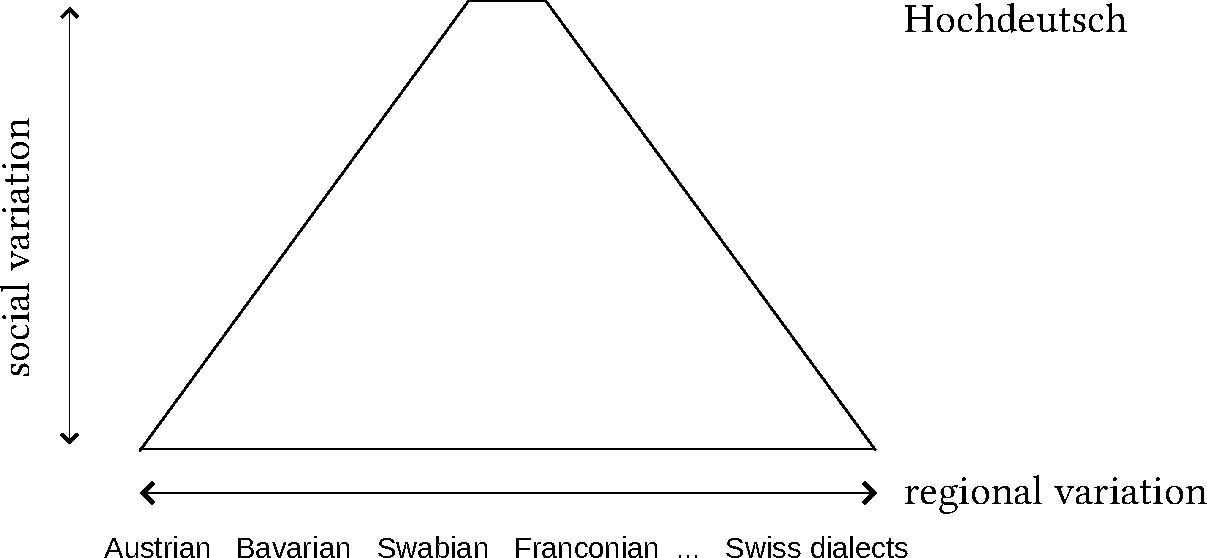
\includegraphics[width=0.8\textwidth]{dollinger-img001.pdf}
\caption{Visualizing the dominant concept of standard German “Hochdeutsch” \citep[40]{Dollinger2019c}}
\label{fig:dollinger:1}
\end{figure}

If Austrian German should be dealt with, Austria would be conceptualized as one such \textit{Stamm} (e.g. \citealt[I: 106]{Kranzmayer1956}), a problem addressed in \citet{Muhr1998}.

While German literature was forced to reorient itself after WWII and replace \textit{Stamm}-based perspectives, there was no complete restart and break in German dialectology between what was done before and after. Language study in German did, in particular, not just continue with pre-war personnel (of whom Kranzmayer in Austria – see below – or Mitzka in Marburg are just two prominent NSDAP members), it has not systematically dehegemonized its conceptions of language. \citet[18]{Auer2013}, for instance, considers the program of \textit{Germanistik} that has been held together by a national perspective of \textit{deutsche Wissenschaft}, as having been replaced after WWII with something else, something more objective. He considers \citegen{Lämmert1967} half-century old account as “still unsurpassed” (\textit{immer noch unübertroffen}). The trope of “bad” dialectology in the Third Reich and “good” dialectology since does not appreciate the problem, however. If \citegen{LämmertEtAl1967} book of four essays is now, more than half a century later, still unsurpassed it would mean that the desiderata, one of which being that “German national identity is based on the assumption of a natural linguistic unity” \citep[34]{Lämmert1967} have not been addressed. Lämmert continues:

\begin{quote}
\foreignlanguage{ngerman}{%
Wann – fragt man sich – werden die Deutschen einer Sprachtheorie entsagen, die sie politisch bereits 1866 widerlegten, mit der sie aber danach noch ein Jahrhundert lang fortfuhren, politische Grenzen je nach Bedarf zu zementieren oder zu negieren? \citep[34]{Lämmert1967}
}\medskip\\
`When – one asks oneself – will the Germans disavow a theory of language, which was politically obsolete in 1866, yet they have continued to operate with for another century, as needed, to buttress or to quash political boundaries?' (translation SD)
\end{quote}

\citet[34]{Lämmert1967} describes OSGA without naming it and sees its rationale in a “particularly rigorous foundation of German national identity in the assumption of a natural linguistic unit of the nation” \footnote{{}“\foreignlanguage{ngerman}{besonders nachdrückliche Fundierung des deutschen Nationalbewußtseins auf der Annahme einer naturgegebenen Spracheinheit der Nation}”}.

Today, of course, no one would adopt such wording. Many, however, take it for granted that the German language is unified, with one standard, or at least one standard that is more equal than all others, and therefore reify resistance against multiple standards. These assumptions, whether expressed or not, come with heavy historical baggage, as they were developed by philologists who subscribed to a pan-German perspective, in which Austria is a key ``possession'', while Luxembourg was not (see \citealt{Dollinger2024} for a most extreme case). 

The very long-reach of a \textit{Stamm}-based concept in German dialectology is reflected in very modern perspectives. We can see it unintentionally expressed in approaches of current cross-border scenarios with German. One notices in \figref{fig:dollinger:2} a disparity in the treatment of borders between Netherlandic Dutch (NL) and German (D) in \figref{fig:dollinger:2a}, and the treatment of the Austrian-German border in Bavaria in \figref{fig:dollinger:2b}. Relying on \citeauthor{Scheuringer1990a}'s (\citeyear{Scheuringer1990a, Scheuringer1990b}) non-quantitative traditional study of that border (see \citealt[42--47]{Dollinger2019c}), the interpretation seems to unwittingly follow the spirit of OSGA, as Munich and Vienna are heteronomous to a joint, cross-border super-regional standard whose sole legitimacy is the Bavarian \textit{Stamm} and dialect zone from a millennium ago.

\begin{figure}
\begin{subfigure}{\textwidth}
  \centering
  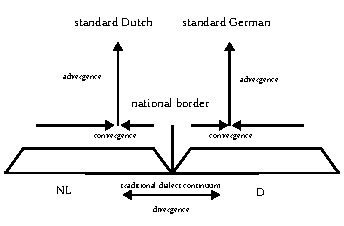
\includegraphics[height=.25\textheight]{dollinger-img002.pdf} 
  \caption{}
  \label{fig:dollinger:2a}
\end{subfigure}
\smallskip\\

\begin{subfigure}{\textwidth}
  \centering
  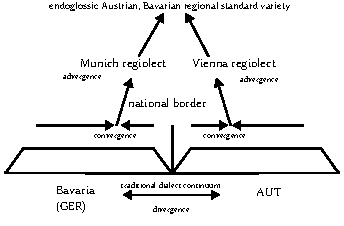
\includegraphics[height=.25\textheight]{dollinger-img003.pdf} 
  \caption{}
  \label{fig:dollinger:2b}
\end{subfigure}
\smallskip\\

\begin{subfigure}{\textwidth}
  \centering
  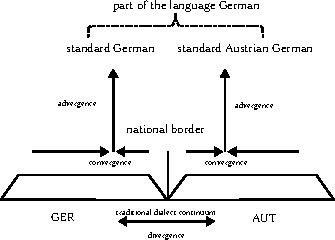
\includegraphics[height=.25\textheight]{dollinger-img004.pdf} 
  \caption{}
  \label{fig:dollinger:2c}
\end{subfigure}

\caption{The NL-D (after \citealt[21]{Auer2005a}; \ref{fig:dollinger:2a}) and AUT-GER borders (\citealt[27]{Auer2005a}; \ref{fig:dollinger:2b}); \citegen[54--58]{Dollinger2019c} reinterpretation (\ref{fig:dollinger:2c})}
\label{fig:dollinger:2}
\end{figure}

\figref{fig:dollinger:2b} therefore shows the long reach of what may be considered a discriminatory concept of language, as Austria and Switzerland appear under OSGA’s umbrella. Pluricentric Theory, however, predicts linguistic diversification across political borders (e.g. \citealt{Kremer1979,Boberg2000}), though \citegen{Scheuringer1990b} qualitative study is not the kind of study that would allow the detection of such diversification as it is too coarse. When, for instance, the geographical dialect continuum between The Netherlands and Germany was disrupted, the “cohesive social system between locations across the state border diverged after the establishment of the state border in the area in 1830, and as a result, so did the dialect variation” \citep[133]{DeVriendEtAl2009}. Any other outcome would, in the light of cross-border evidence, be surprising. The same process would be expected to apply at the Austrian-German border.

Historically, German dialectology operated with tropes of domination, which can be seen, for instance, in Anton \citet[58]{Pfalz1927} – Kranzmayer’s superior from 1926 to 1937 at the Vienna dictionary project – who insisted that a difference must be made between dominant and non-dominant \textit{Stämme} and that Saxons and Franks in Austria would be “fully Bavarianized in short periods of time” [“in kurzer Zeit vollständig baiwarisiert”] \citep[60--61]{Pfalz1927}, the dominant \textit{Stamm}. The theme of dominance was big in \textit{völkisch} linguistics. The dominant \textit{Stämme} win and dominate others and therefore further improve the German race, the argument goes. The idea of \textit{Stämme} is central and Germanistik has “frequently improved” \textit{deutsche Volkskunde} in the “spirit of the Grimm Brothers” \citep[62]{Pfalz1927}. While this kind of discourse has stopped, the frame of OSGA carries over this trope of domination in which one standard ``tames" all other varieties.

It needs to be noted that there is no structural difference between Nadler’s application of \textit{Stämme} to literature and the application of \textit{Stämme} to language, shown in Figures~\ref{fig:dollinger:1} and \ref{fig:dollinger:2}b. \textit{Stämme} continue to be treated as relevant in linguistics and the varieties of the various \textit{Stämme} are considered hyponyms to Standard German, under the OSGA umbrella. While historical accounts speak of Old High German as having had “no uniform linguistic entity”, “but a series of more or less clearly demarcated dialects that are lumped together under the umbrella term [Old High German]“\footnote{{}``keine einheitliche Sprachform'', ``sondern aus einer Reihe von mehr oder weniger deutlich voneinander abgegrenzten einzelnen Dialekten bestand, die unter diesem Oberbegriff zusammengefasst werden.''} \citep[76]{Ernst2021}, current conceptualizations of present-day German refer to these dialect zones and foreground them in interpretations: “It is frequently seen that [present-day] variants surprisingly clearly coincide with the old dialect zones; occasionally there are unexpected alignments”\footnote{{}``Allerdings zeigt sich häufig, dass … Varianten erstaunlich deutlich mit den alten Dialekträumen übereinstimm[en], hin und wieder ergeben sich unerwartete Allianzen.''} \citep[73]{ElspaßEtAl2017}. Elspaß' interpretations such as the one above leave the \textit{Stamm}-based model intact and conceptually and constructively unchallenged. In Third Reich diction, Nadler considered \textit{Stämme} as the immutable \textit{sine qua non}: “There is no race history in the humanities that does not take note of the indisputable fact of \textit{Stämme}”\footnote{{}``Es kann keine geistesgeschichtliche Rassenkunde geben, die nicht von dem unabweisbaren Tatbestand der Stämme Kenntnis nehme.''} \citep[18]{Nadler1934}. While very different in application, the basic, field-defining construct of \textit{Stämme} remains unchallenged and only the language historian occasionally refers to the arbitrary linguistic demarcation that has become disciplinarily, conceptually enshrined and has, as Elspaß’ intepretations illustrate, become the default expectation today.

\citet[78]{Hutton1999} points out that treating \textit{Stämme} as objective analytical units has advantages. It “preserves disciplinary history intact, for it relegates Nazism to the non-scientific realm, to that of the methodologically aberrant”. German dialectology has not been willing to engage in this disciplinary argument (see, e.g. \citegen{Langer2021} review of \citealt{Dollinger2019c}) and clearly prefers a ``pluri-areal", non-pluricentric approach to German. When today someone argues that Austria is no single dialect zone (95\% Bavarian dialects, but some Alemannic too), and therefore there cannot be an Austrian Standard German (e.g. \citealt[50]{ElspaßNiehaus2014,Herrgen2015,Elspaß2020}), they unwittingly engage in acts of language making that reconfirms the conservative focus on one standard of German under OSGA.

\section{Pluricentric theory plus three fail-safes}
\label{sec:dollinger:3}
\textit{Stamm}-based approaches are static conceptions of German that, while permitting the tweaking of the one standard, do not allow for the development of newer standards. In its guise as “pluri-areal” \citep{ElspaßEtAl2017}, they sound similar to pluricentric theory, yet as basically \textit{Stamm}-based ideas of the German language they cannot effectively adapt to developments since the 1800s, e.g. such as transcultural influences. A single standard for German, often in the term \textit{standard German}, remains the linguistically dominant perspective at the beginning of the 2020s.

Linguists may, for instance, document respondents’ doubt in Standard Austrian German rather than interpreting doubts as expressions of linguistic insecurity (e.g. \citealt{KoppensteinerLenz2020}), a concept well established in English dialectology \citep{Preston2013}, a concept essential in non-dominant varieties such as Austrian German, yet a concept not used in German dialectology. Researchers may unwittingly engage in acts of language unmaking and become non-con\-sent\-ing agents of OSGA via the disciplinary legacy of German dialectology. For instance, in the Swiss context \citet[60]{Dürscheid2009} considers the standard of Germany as the usual ``benchmark”, not Standard Swiss German. Senior Marburg researchers proclaim an entirely new era in German language history, without recourse to linguistic insecurity, and see “de-nationalization” as “a new phase for the standard norm” \citep[156]{Herrgen2015}. Pluricentricity, however, is considered as “an entirely political concept” \citep[50]{ElspaßNiehaus2014}, while the political dimension of the notion “German” is not addressed. Instead, bottom-up aggregate approaches render the state border a-priori as irrelevant. Methodologically, a dozen pre-defined areas comprise the German-speaking lands, stripping the national identity level of its relevance by demanding categorical differences on each side of the national border (e.g. \citealt[52]{Elspaß2020}).

What is methodologically reified is the construct German (it is what is fed the algorithm); what is voided are younger standard varieties such as Austrian or Swiss German, nipping Standard South Tyrolean German pre-emptively in the bud. An insensitivity to the social salience of variables leads to assessments such as “[l]ess than two per cent of variation in standard German … does hardly make a ‘variety’” \citep[50]{ElspaßNiehaus2014}, while, in fact, it is up to the speakers to decide how to view their code. Such statements should be seen as blatant statements of language making and unmaking, not as disinterested analysis. For good reason, \citet[383]{Ruck2023} pleads for the inclusion of a language political angle in German studies curricula that would, among other things, reveal such disciplinary biases. Approaches such as \citet{Muhr2017} or \citet{DeCilliaRansmayr2019}, clearly in a minority today in the light of ``Deutsch in Österreich'' Special Research Clusters, are aware of language political imbalances and aim to mitigate linguistic insecurity in Austria.

As such, the 2020s are in stark contrast to a generation earlier, when Michael \citet{Clyne1995}, Peter \citet{vonPolenz1994} and Ulrich \citet{Ammon1995} brought pluricentric concepts for a short time into the mainstream of German dialectology. A logical consequence of ignoring the autonomy of Standard Austrian German (cf. \citealt[9--12]{ChambersTrudgill1998}) and of supporting anti-pluricentric approaches in the 2010s is \citegen{Muhr2021} call for an ``Austriazistik'' – Austrian Studies – that is independent of \textit{Germanistik} – German Studies. Which model of language would be most conducive to accommodate the changing nature of present-day varieties? It is likely not the monocentric model in \figref{fig:dollinger:1}, unchanged in its conceptions for centuries, and stuck in a past where one German-speaking state seemed possible, indeed desirable. This is the ``pluri-areal" model.

 The model of language that seems open for expansion and adaptation is, however, the pluricentric model. It is the default setting in English linguistics (with particular focus on World Englishes) and the model that was applied by \citet{Clyne1995} to German. The term \textit{center} is to be understood in a metaphorical manner, not a precise location. \citet{Auer2021} suggests the term “multiple-standard language” rather than pluricentric language in order to avoid this confusion. It is useful to visualize the pluricentricity -- multiple standards -- of German schematically in “Trudgill’s pyramids” as follows (\figref{fig:dollinger:3}).

\begin{figure}
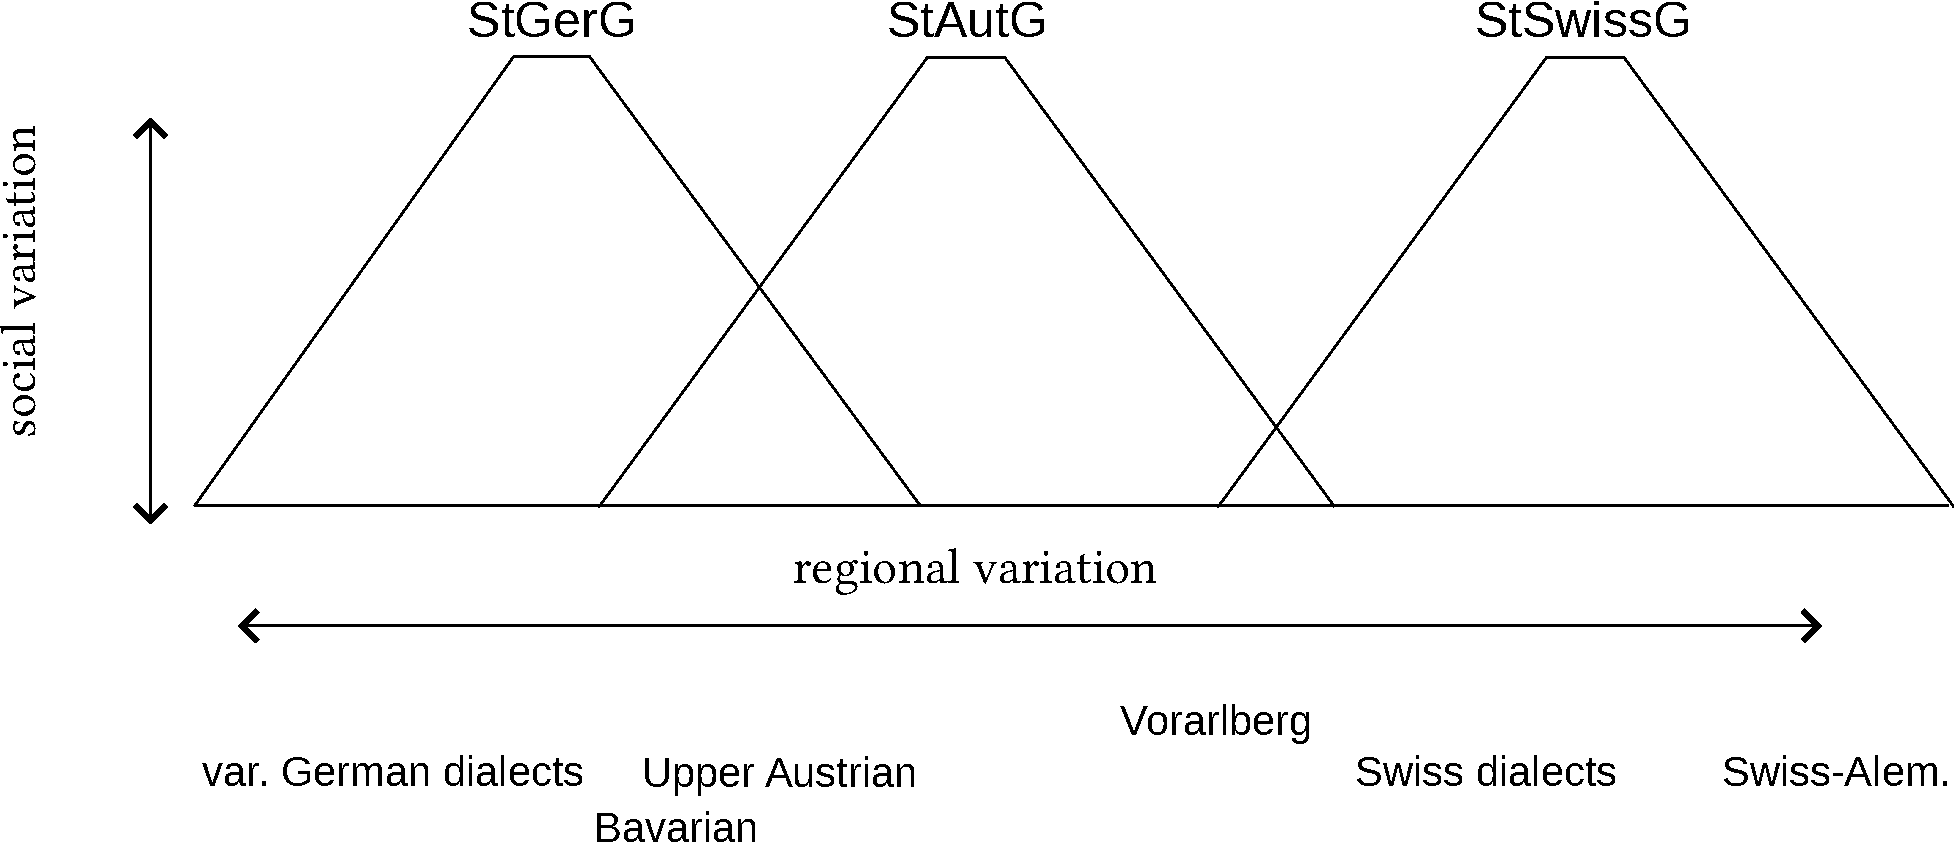
\includegraphics[width=\textwidth]{dollinger-img005.pdf}
\caption{Visualizing multiple standards of German (modeled after \citegen{Trudgill2000} pyramid concept; \citealt[39]{Dollinger2019c})}
\label{fig:dollinger:3}
\end{figure}


On the horizontal plane, the model shows regional non-standard variation. This feature overlap – often used as an argument against Standard Austrian German – is built into the pluricentric model. It predicts, for instance, that the regions of Bavaria in Germany and Upper Austria share more non-standard features with one another than Vorarlberg and Upper Austria. It does not employ, however, the millennium-old level of \textit{Stamm}-based dialects and thus avoids the unmaking of younger standards, such as the Austrian or Swiss standards. Social variation is depicted on the model’s vertical axis, variation that may also be situationally dependent: Speakers may use Standard Austrian German where the context requires it (top of pyramid), dialects when appropriate (base of pyramid), or intermediate forms (\textit{Umgangssprache} `colloquial language') somewhere in between.



The pluricentric model is open to modifications. For instance, the influence of varieties cross-linguistically (e.g. \citealt{BuschfeldKautzsch2020,Schneider2022}), can be shown visually as a cross-bar that covers all three varieties. Transnational influences from additional contexts and varieties may be depicted by bars of different colours cutting across a particular pyramid, a pair, or all three. For instance, as global English terms spread via socially upper or intermediate strata, a “bar of Global English” (e.g. \textit{die Compliance}, \textit{das Tool} from business German, or \textit{chillen, slayen, texten, SMSen} from youth language) cut across the upper middle of all three pyramids without, and this is key, dissolving each pyramid’s reference point of an autonomous standard (\figref{fig:dollinger:4}).



Adaptations specific to a particular variety may also be visualized in different shapes of the pyramid. For instance, the wider functional range of Swiss dialects as used in TV talk shows or on radio compared to Austrian (and German) ones may be reflected in a broader x-dimensional box of the dialects on the y-axis, as shown in \figref{fig:dollinger:4}. Influences from Germany on the smaller standards (e.g. <-ig> pronounced as /iç/ and not as /ig/, \textit{Eimer} for \textit{Kübel} ‘bucket’) may be depicted by arrows spreading out from Germany into Austria and Switzerland. Vice versa, reverse influence (e.g. \textit{es geht sich (nicht) aus} – an AutG expression denotating ‘it suffices / does not suffice’) would be shown by, perhaps thinner because less forceful, arrows. These adaptations are possible without diminishing the identity-affirming frame of standard varieties for some (small) nations, as they maintain national priming effects, which may also serve as identity markers. They visualize \citegen{Schneider2022} suggestion of “epicenters” in one country that may influence other centers but do not hegemonize smaller standards and frames by virtue of differential speaker numbers (e.g. 83 million Germans vs. 9 million Austrians).


\begin{figure}
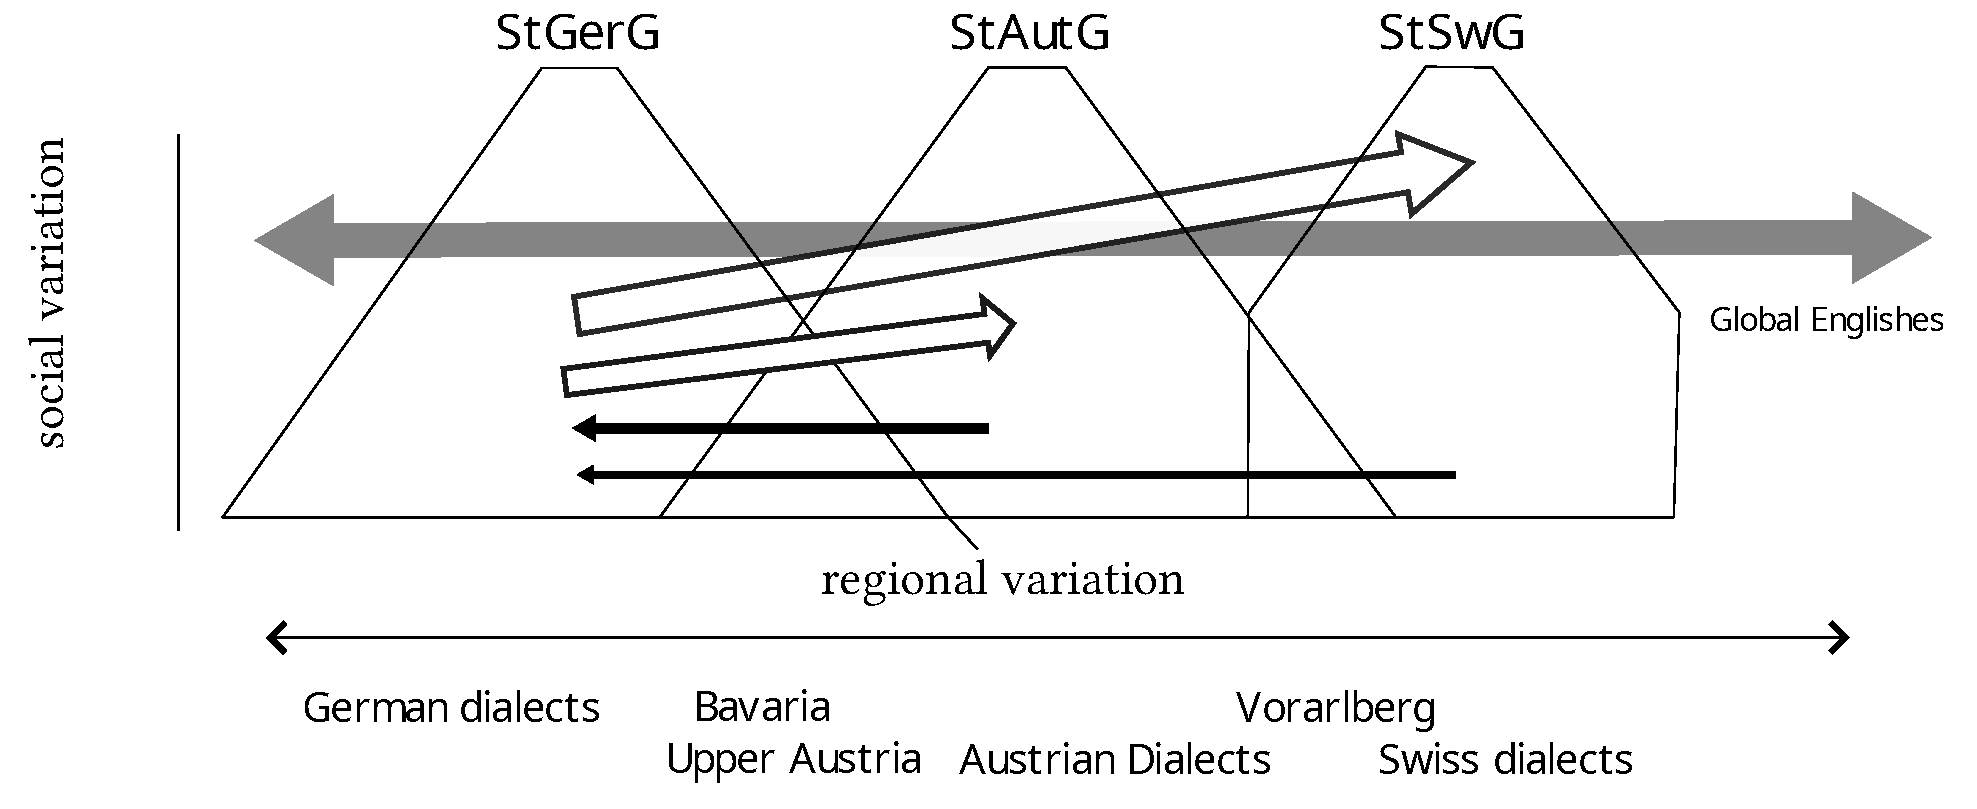
\includegraphics[width=\textwidth]{dollinger-img006.pdf}
\caption{Pluricentric, multi-standard model of present-day German, with inter-language and global influences visualized by arrows}
\label{fig:dollinger:4}
\end{figure}

The model can be extended when new standards emerge, as may happen with South Tyrolean German once it features a codified dictionary \citep{Hofer2020}. The pluricentric model also allows the maintenance of reference frames that function as identity markers in international contexts. While dialects and \textit{Umgangssprache} (colloquial language) are identity markers domestically or in some cross-border contexts (e.g. Upper Austria and Bavaria), in the international or EU context the standard varieties take on this function (e.g. \citealt{DeCilliaEtAl2020} for language and identity in Austria).


\section{Three fail-safes against linguistic hegemony} 
\label{sec:dollinger:4}
Three ``fail-safes" are suggested to mitigate the inadvertent effects of linguistic hegemonic discourse in German dialectology. They would allow the detection of obsolete language conceptions for present-day speakers. They would support the implementation of Lämmert’s half-century-old suggestion to discard the traces of linguistic domination in the concept of German. They may be used in connection with the pluricentric model to see where further refinement is needed. The three fail-safes (\cites{Dollinger2019b}[107--114]{Dollinger2019c}) are rooted in the goal of increasing the relevance of dialectology and linguistic study for as many speakers as possible while avoiding the sociolinguistic language unmaking of non-dominant (Austria, Switzerland), perhaps not fully developed (e.g. South Tyrol), standards, or their demotion to one of 15 all-German-language regions (e.g. \citealt{DürscheidElspaß2015}).


\subsection{The speaker is always right (fail-safe \#3)}
\label{sec:dollinger:4.1}
In addition to linguistic production data, language attitudinal data needs to be considered, even foregrounded.  \citet[137, Abb. 36]{DeCilliaRansmayr2019} show that in Austria 80\% of secondary school students, and 90\% of their teachers, perceive “more than one standard in German”. This pluricentric perspective is currently not appropriately reflected in German dialectology. From a sociolinguistic perspective, the current anti-pluricentric approach violates fail-safe \#3, which is “the speaker is always right” \citep[113--114]{Dollinger2019c}. That is, the \textit{informed} speaker, who has been briefed about the construction of standard varieties and their reifying nature, is always right. As \citegen{DeCilliaRansmayr2019} results show, the need for Standard Austrian German is not diminishing. Such results are in clear contradiction to the Marburg School’s verdict of the “de-nationalization [\textit{Entnationalisierung}] of German” \citep[157]{Herrgen2015}, which is based on a methodologically questionable assessment of Austrian listeners ranking the standard speaker from Germany a tiny bit more “pure Hochdeutsch” than the Austrian one \citep[154]{Herrgen2015} (see for a detailed critique \citealt[78--84]{Dollinger2019c}).



\citegen{DeCilliaRansmayr2019} results, in contrast, may be considered a mandate for \textit{Germanistik} to reconsider the relevance of its language models for speakers beyond Germany. It would imply that we need to, in Labovian ways, mitigate linguistic insecurity appropriately and inform speakers of the possibilities. For instance: “You don’t need to try to sound like someone from Hanover when you speak standard.” If after such information the speaker prefers a Northern German model, we can rest assured that our data is valid. The speaker is, after all, indeed always right, and the primary problem here is to assess which majority of speakers is given credence. Paramount is the sociohistorical embedding, which, in the Austrian context, is one of ridicule and linguistic insecurity.



Current practice is rather the opposite, however, as the bar for a newer Austrian standard is set unreasonably high by German dialectologists. When, for instance, \citet[66]{Elspaß2020} states that a given feature is dominant but not “absolute” in Austria – meaning, in a crude dichotomy, that the feature is not \textit{exclusively} used in Austria – and that thus there cannot be a Standard Austrian German, the bar for acceptance of Standard Austrian German is lifted so high that very few established languages on earth would ever clear it.


\subsection{Work with explicit, falsifiable theories (fail-safe \#2)}\label{sec:dollinger:4.2}

Fail-safe \#2 \citep[111--113]{Dollinger2019c} calls for explicit, falsifiable theories. Pluricentricity is such a theory, as, for instance, it makes predictions of how language variation across political borders develops. It predicts, among other things, that the varieties on either side of an arbitrary political boundary will diverge depending on a list of factors (e.g. \citealt[29]{Auer2005a}). It predicts that there will be, often considerable, feature overlap (e.g. Bavaria and Upper Austria in \figref{fig:dollinger:2}), yet the same or near-identical features will be framed differently, depending on which side of the border one is positioned (geographically, socially, attitudinally and cognitively).

``Pluri-areal" creed, by contrast, offers no theory; it does not make falsifiable predictions. It is synonymous with unspecified geographical variation and equivalent with the term “anti-pluricentric” \parencites[103--106]{Dollinger2019b}[62--176]{Dollinger2019c}. This distinction is important, because the statement that German is a ``pluri-areal" language, a language with geographical variation, cannot be falsified. As that view does not specify in which ways this variation occurs, it cannot make predictions; it cannot do more than to negate pluricentric theory. Paradoxically, ``pluri-areal", however, is presented as on a par with pluricentric theory and, in most cases, as superseding the pluricentric approach (e.g. \citealt{DürscheidElspaß2015,ElspaßEtAl2017,Langer2021,DiÖ2021,MeerDurgasingh2025}).

Pluricentric predictions include, for instance, that linguistic production will diversify with the duration of the political division at a given border. They are testable and falsifiable. In this context, I would like to correct the assessment that pluricentric approaches “lend themselves to nationalistic views and exploitations because they are interested predominantly in linguistic perception rather than production” \citep[470--471]{Schneider2022}. While perception and the cognitive frame of speakers certainly play an important role in Pluricentric Theory, production is not unimportant, though it is not the sole criterion – as it is in most ``pluri-areal" studies – for lumping varieties together as a language. The proof that anti-pluricentric perspectives are not theoretically anchored can be taken via Karl Popper’s epistemological concept (explored in \citealt[89--90]{Dollinger2019c}), or with \citegen[169]{Lewin1952} \textit{bon mot} that “there is nothing more practical than a good theory.” This practical angle of pluricentric theory – as applied to Standard Austrian German – can be seen, for instance, in German as a Second Language teaching in Austria, where German-made material is often irrelevant, or, at least, inappropriate. A first-hand report is from a German Beginner Textbook by Hueber \citep[59--60]{Dollinger2021}, which in the first week was dealing with a difficult phonetic distinction -- <ä> vs. <e> or /ę/ vs. /e/ -- that is near-categorically absent in Standard Austrian German and even in Germany a stylistic and not a phonemic distinction. Likewise, professional translators and interpreters universally understand and appreciate the necessity of the concept of Standard Austrian German, as seen in recent movies such as \textit{Rush} (\citeyear{Howard2013}) which portrays the life of Formula~1 star Niki Lauda, with German actor Daniel Brühl, playing the Austrian Lauda, getting lessons on SAutG, thus rendering the movie quite authentic.

\subsection{Uniformitarian Hypothesis: Vertical and horizontal readings (fail-safe \#1)}\label{sec:dollinger:4.3}

From a sociolinguistic angle perhaps the most powerful argument for the consequent adoption of a pluricentric perspective in mainstream German dialectology can be made via the Uniformitarian Hypothesis.  Fail-safe \#1 \citep[109--111]{Dollinger2019c} calls for theorizing to be in line with both the vertical and horizontal readings of the Uniformitarian Hypothesis (e.g. \citealt[21]{Labov1994}). What I call the \textit{vertical} reading of the Uniformitarian Hypothesis is common practice in historical linguistics. Linguists assume, all other things being equal, that the language change of the past must have proceeded in a similar manner to the change of the present. The vertical, the diachronic, reading is universally accepted as one of the theoretical anchors of historical linguistics.

In addition to this well-known vertical (diachronic) reading, I would like to formalize a synchronic, a horizontal reading. The horizontal reading of the Uniformitarian Hypothesis \citep[110--111]{Dollinger2019c} can be described as follows: If two languages have comparable cross-border situations, codifications and social scenarios, they \textit{must} be modeled the same way unless there are salient differences. Such equivalent situations exist, for instance, for American/Canadian English, Dutch/German or Austrian German/German German. Recent models of Netherlandic Standard Dutch and Belgian Standard Dutch (e.g. \citealt{DeRidder2020}) underscore via horizontal uniformitarian comparison the distinction between Austrian Standard German and German Standard German. In other words: What applies to the sociolinguistic goose, must also apply to the sociolinguistic gander. If we model younger standard varieties, such as Canadian English or Belgian Dutch, in one way, with two autonomous standard varieties, we \textit{must} model the Austrian-German context in like manner.



\begin{table}
\footnotesize
% \begin{tabularx}{\textwidth}{lQQQQQQ}
% \lsptoprule
% & A) & B) & C) & D) & E) & F) \\
% & {Conditions for codification} & {How many speakers see a distinct variety?} & {Linguistic} {insecurity} {today} & {Codification} & {Academic} {interest}  & {History}\\
% \midrule
%  {CanE} & after WWII & 80\% \citep[234]{Dollinger2019a} & Somewhat, decreasing & {First general dictionary 1937} & increasing & Canada as colony till 1866\\
%  & & & & Full-size dictionaries 1962--1967  & & \\
%  \midrule
%  {AutG} & after WWII & 80--90\% (\citealt{DeCilliaRansmayr2019}: Abb. 36) & Somewhat, possibly increasing & \citet{Lewi1875} \citet{Wittgenstein1926}
%  \citet{ÖWB1951} & decreasing & Austria leader of German states till 1866\\
% \lspbottomrule
% \end{tabularx}
\begin{tabularx}{\textwidth}{lQQQ}
\lsptoprule
& & CanE & AutG \\
\midrule
A) & Conditions for codification & After WWII & After WWII \\
\midrule
B) & How many speakers see a distinct variety? & 80\% \citep[234]{Dollinger2019a}  & 80--90\% (\citealt{DeCilliaRansmayr2019}: Abb. 36) \\
\midrule
C) & Linguistic insecurity today & Somewhat; decreasing & Considerable \\
\midrule
D) & Codification & First general dictionary 1937, full-size dictionaries 1962--1967  & \citet{Lewi1875}, \citet{Wittgenstein1926} \citetitle{ÖWB1951}\\
\midrule
E) & Academic interest & Increasing & Decreasing, but substantial for ``German in Austria"\\
\midrule
F) & History & Canada as colony until 1866 & Austria leader of German states until 1866\\
\lspbottomrule
\end{tabularx}
\caption{Sociolinguistic benchmarks for assessment with the Uniformitarian Hypothesis, horizontal reading}
\label{tab:dollinger:1}
\end{table}

\tabref{tab:dollinger:1} is a comparison of basic benchmarks in Austria and Canada regarding the non-dominant status of German and English. With only some key benchmarks showing, it gives an example of the horizontal reading of the Uniformitarian Hypothesis. The social conditions for codification were fully present after World War II in both countries (Row A). At this point, Canada became de-facto independent from the UK (issuing their own passports as of 1947). Austria had by that time overcome the Third-Reich unification with Germany which resulted in a renewed focus on Austrian dimensions. Row (B), how many speakers recognize a distinct variety, is important, with clear majorities in both countries around the 2010 polling dates. This language awareness is a process and in 1945, the answers would have looked different.\pagebreak

In light of \tabref{tab:dollinger:1}, an argument would need to be brought forth \textit{against} the younger standard varieties of Austrian German and Canadian English today and not \textit{for} them. \figref{fig:dollinger:2b} is therefore remarkable as it breaks, without a discernible rationale, with the horizontal reading of the Uniformitarian Hypothesis and suggests that Austrian and German represent some sort of special case. A \textit{Sonderweg} seems to be invoked by those German linguists who address the issue (e.g. \citealt{Glauninger2013}), while most seem to unwittingly apply a treatment in violation of the horizontal reading of the Uniformitarian Hypothesis and in compliance with OSGA.

\section{Conclusion}\label{sec:dollinger:5}

The suggested three fail-safes combined would considerably reduce lingering disciplinary hegemonic perspectives that constitute some form of language unmaking. They would curb cyclical interpretations of data – studying German means that any approach confirms the existence of one German (OSGA). Since 2010, the rhetoric against pluricentricity has gotten markedly more aggressive (see for a summary \citealt[139--159]{Dollinger2021}). In comparison to other dialectological fields such as Portuguese, followed by English, Spanish, and even French (where skepticism to multiple standards has a long tradition, see \citealt{Oakes2001}), German dialectology is today the \textit{most} conservative in its language modeling (see \citealt{Dollinger2023a}). Multiple standards of German are, for instance, downplayed as irrelevant (e.g. \citealt[245]{BeschWolf2009}), denied their existence (Stephan Elspaß, quoted in \cites[10]{Muhr2020b}[50]{ElspaßNiehaus2014}), or at least put into question (\citealt[48,74]{KoppensteinerLenz2020}). I have attempted to show that such questions are in the last instance, harking back to \citet{Lämmert1967}, the unintended result of undetected field-internal pan-German frames of reference. The question is, therefore, to what degree German dialectology is still influenced by underlying, pan-German presuppositions today. If the \textit{Germanistik}-internal resistance against Standard Austrian German, a trope in the field since at least 1951 (e.g. \citealt[500--502]{Muhr2020a}), is taken as a measure, the influence is considerable and warrants its own name, for which I suggested the “One Standard German Axiom” (OSGA). OSGA has been an underlying assumption, a driving force in German dialectology and linguistics since Grimm’s day, whether explicit (until about 1960), or implied (since then).


From such a backdrop, it is clear why language teachers of German outside of Germany understand the \textit{sine qua non} of Pluricentric Theory (e.g. \citealt{CalliesHehner2023}). \citet{Ruck2021}, in German didactics, is a positive review in obvious contradiction to \citegen{Langer2021} utmost dismissal of \citet{Dollinger2019c}. Pluricentricity is, using Lewin’s phrasing, a most practical theory -- a theory that applies, as any linguistic theory should, cross-linguistically. The long-standing resistance against Standard Austrian German is deep-rooted in German linguistics. It applies a threshold that keeps being raised, in its most recent reiteration, by Elspaß, for example. If in 1800 German had had that bar as high as it is now, there would be no such language today. Standard varieties do not just emerge bottom-up, they are also shaped top-down. German dialectology has been one top-down player in the language making process, as are national education boards, national broadcasters and a range of other agents.


I have argued that a One Standard German Axiom has been at the core of work in German dialectology -- a presupposition that goes back to pan-German thought. While no present-day linguist has anything to do with this period or thinking, it was a different matter for some of their teachers and teachers’ teachers (e.g. the cases of Kranzmayer or Mitzka). This continuity in German linguistics has already been reconstructed from the disciplinary record, e.g.  \citet[1--2]{Hutton1999}, who looked at the connection of German linguistics and anthropology. While today there are clear differences to the past in a number of important ways, the answer to lingering conceptual continuities seems to lie in field-internal presuppositions that have been passed down through generations of researchers, from the Humboldtian tradition (which “puts prime emphasis on language as a defining national identity”, \citealt[263]{Hutton1999}), via Weisgerber (the post-WWII “redemption of the German people through their language”, \citealt[143]{Hutton1999}), in the form of a priori assumptions concerning one standard in German. As such, the One Standard German Axiom is an expression of a process of disciplinary language (un)making that has real-life consequences for the speakers of Austrian German and other non-dominant varieties \citep[155--159]{Dollinger2021}. The case for Standard Austrian German is strong. If German dialectology continues to fail to register the relevance of attitudinal findings and speakers’ cognitive identity constructions, it remains conceptually stuck in its pan-German past. De-hegemonization might start with a reformulation of the a priori assumption of how many standards of German there should be presently. The suggested answer is: more than one.


\printbibliography[heading=subbibliography,notkeyword=this]
\end{document}
